\label{chap:dashboard_deployment}

\section{Introduction}
A theoretical algorithm or isolated machine learning script is ineffective in a disaster crisis unless packaged into an accessible, robust, and intuitive software system that emergency managers can operate under extreme stress. First responders, civil defense personnel, and incident commanders require an operational interface where aerial drone imagery can be ingested, analyzed, and synthesized into actionable situation reports within seconds.

This chapter details the software engineering, full-stack architecture, API endpoint designs, and multi-cloud deployment ecosystem of the FloodSense interactive platform.

\section{Full-Stack System Architecture}
The FloodSense platform follows a decoupled client-server architecture designed for high availability, low latency, and cross-platform accessibility. Figure~\ref{fig:deployment_topology} illustrates the cloud deployment topology.

\begin{figure}[htbp]
	\centering
	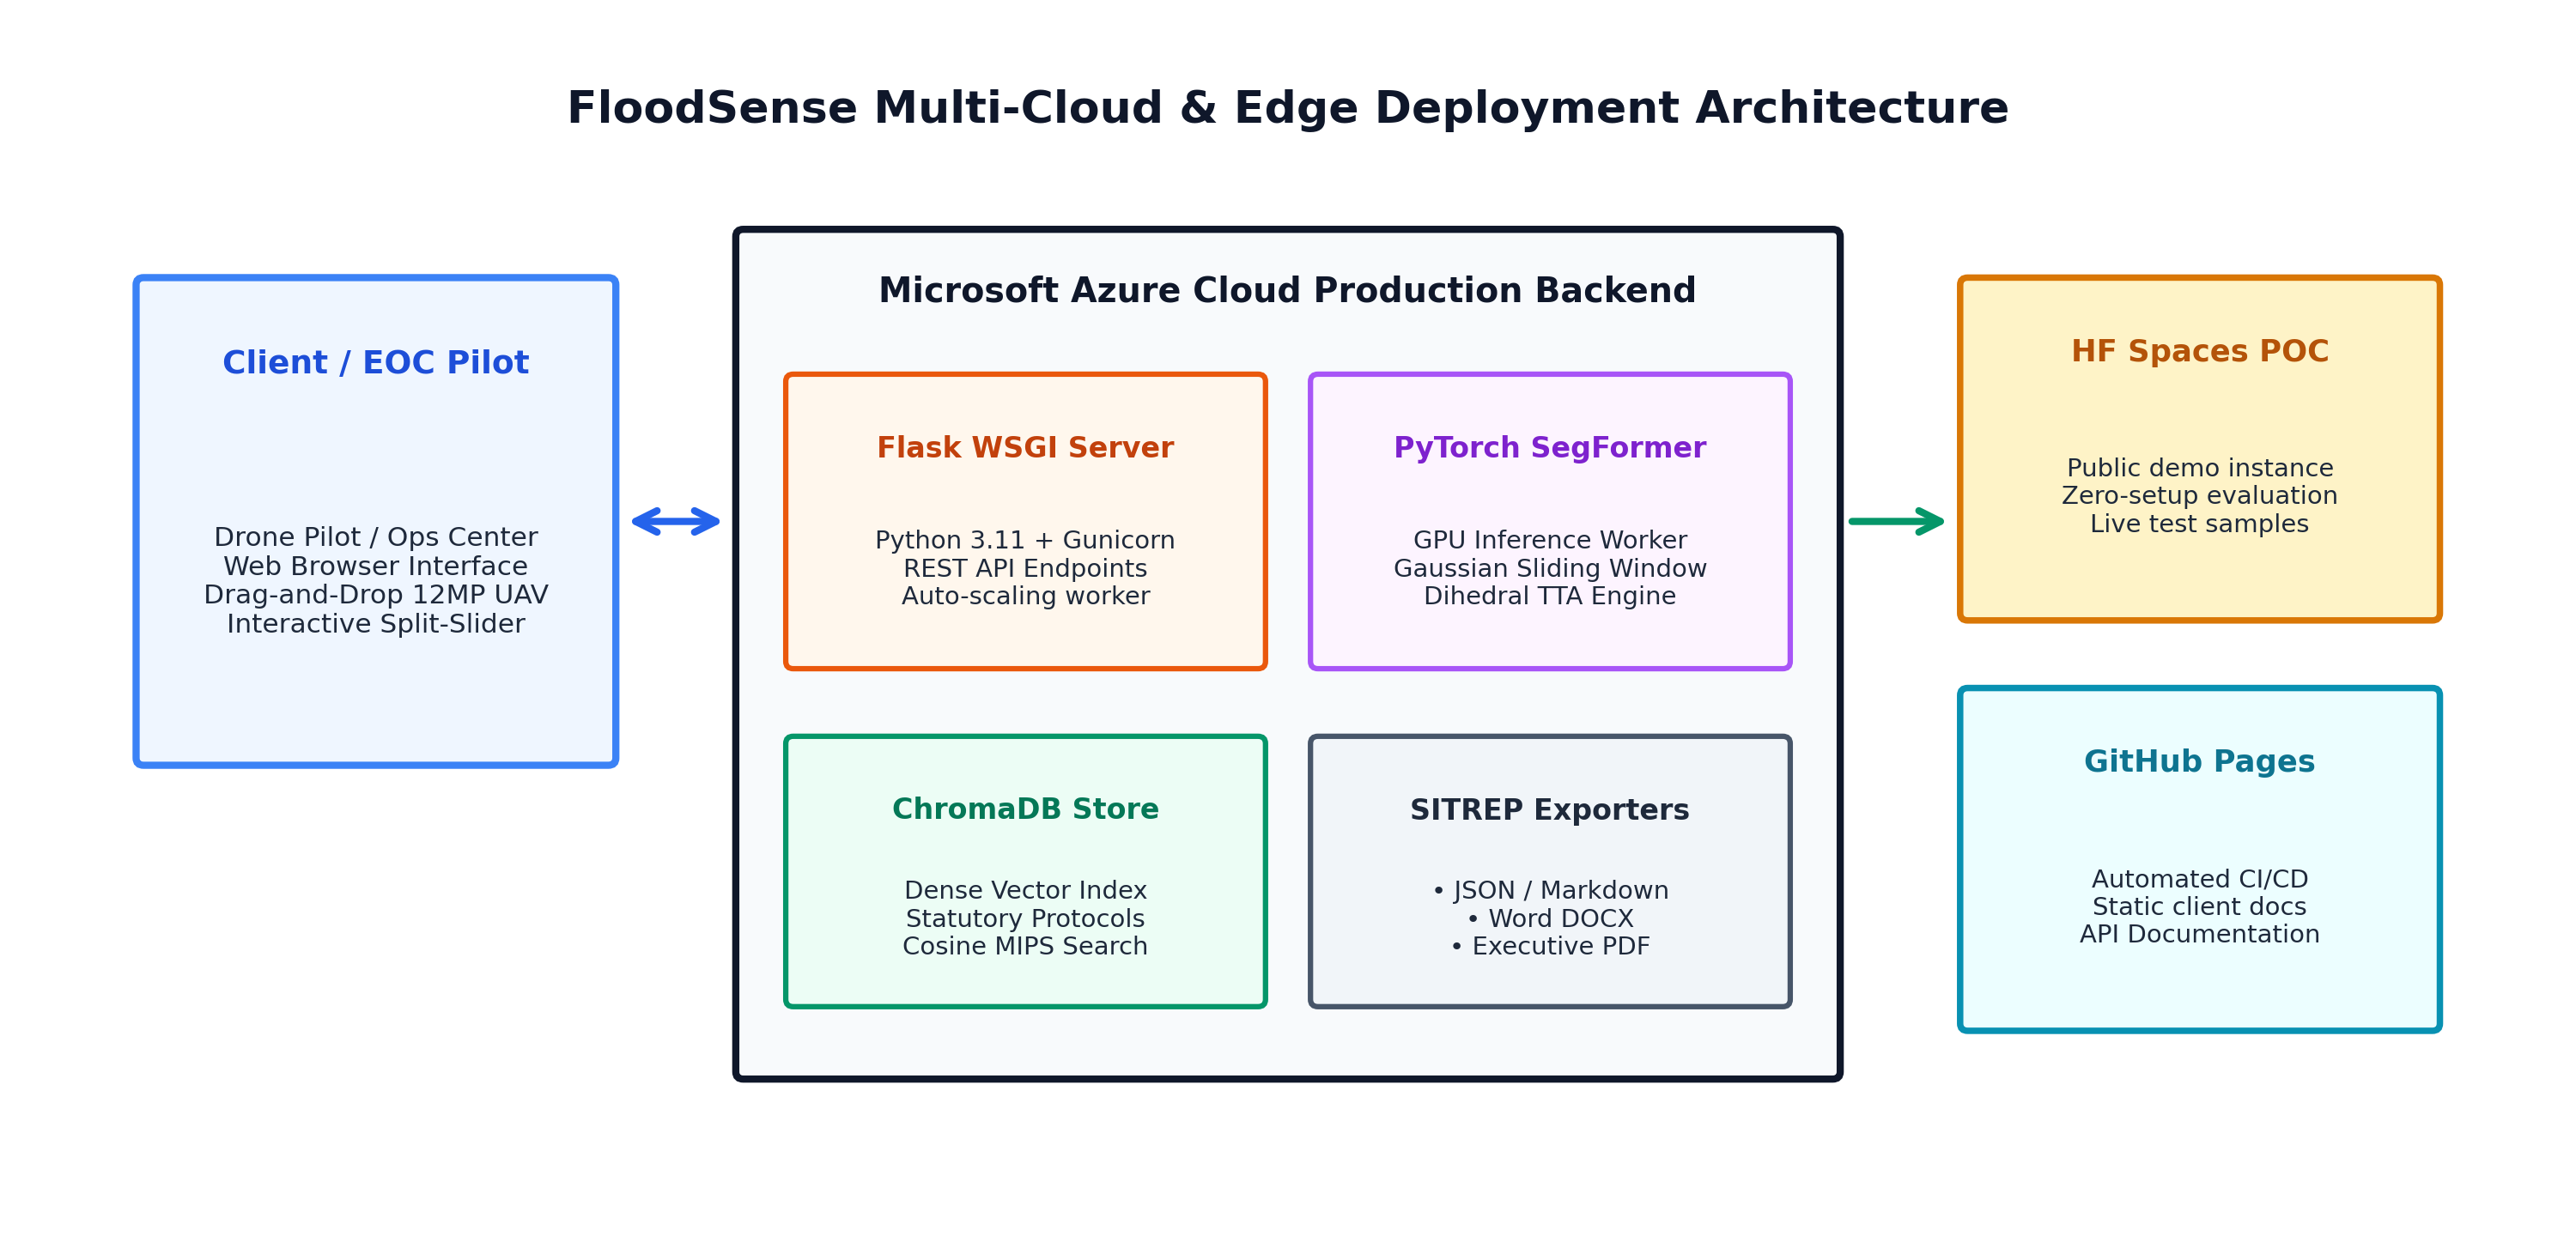
\includegraphics[width=0.92\textwidth]{images/fig7_deployment_topology.png}
	\caption{FloodSense Deployment Topology: Decoupled client-server architecture illustrating UAV data ingestion, WSGI backend processing, vector search, and multi-format report export.}
	\label{fig:deployment_topology}
\end{figure}

\section{Backend Architecture and REST API Design}
The backend service is engineered in Python using Flask and served via Gunicorn for enterprise production concurrency. Implemented in \texttt{dashboard/server.py}, the service exposes a suite of clean, modular RESTful API endpoints:

\begin{enumerate}
    \item \textbf{\texttt{POST /api/segment}:} Ingests a raw drone orthophoto (JPEG/PNG), normalizes tensors, executes the SOTA Class-Balanced SegFormer forward pass (or sliding-window inference), colorizes the predicted 10-class lattice using the FloodNet palette, and returns a high-resolution base64 PNG mask along with per-class pixel counts.
    \item \textbf{\texttt{POST /api/damage\_assessment}:} Consumes the semantic mask, performs morphological connected component analysis, computes the flooded building count, submerged road percentage, and stranded vehicle count, and outputs the composite Disaster Severity Score ($S_{severity} \in [0, 100]$) and emergency priority tier.
    \item \textbf{\texttt{POST /api/retrieve\_protocols}:} Takes damage criteria or free-form natural language queries, performs dense vector cosine search over the ChromaDB vector store, and returns the top-$k$ relevant statutory protocol paragraphs with source document citations and confidence scores.
    \item \textbf{\texttt{POST /api/generate\_sitrep}:} Coordinates the visual metrics and retrieved protocol context through the LLM synthesis engine (or deterministic fallback engine), compiling the formal Situation Report and generating dynamic download URLs for JSON, Markdown, DOCX, and PDF formats.
    \item \textbf{\texttt{GET /api/health}:} Lightweight liveness and readiness probe for cloud monitoring and Kubernetes/Docker health checks.
\end{enumerate}

\section{Interactive Dashboard Frontend}
The user interface is engineered to eliminate cognitive friction during high-stress operations (Figure~\ref{fig:dashboard_ui_mockup}).

\begin{figure}[htbp]
	\centering
	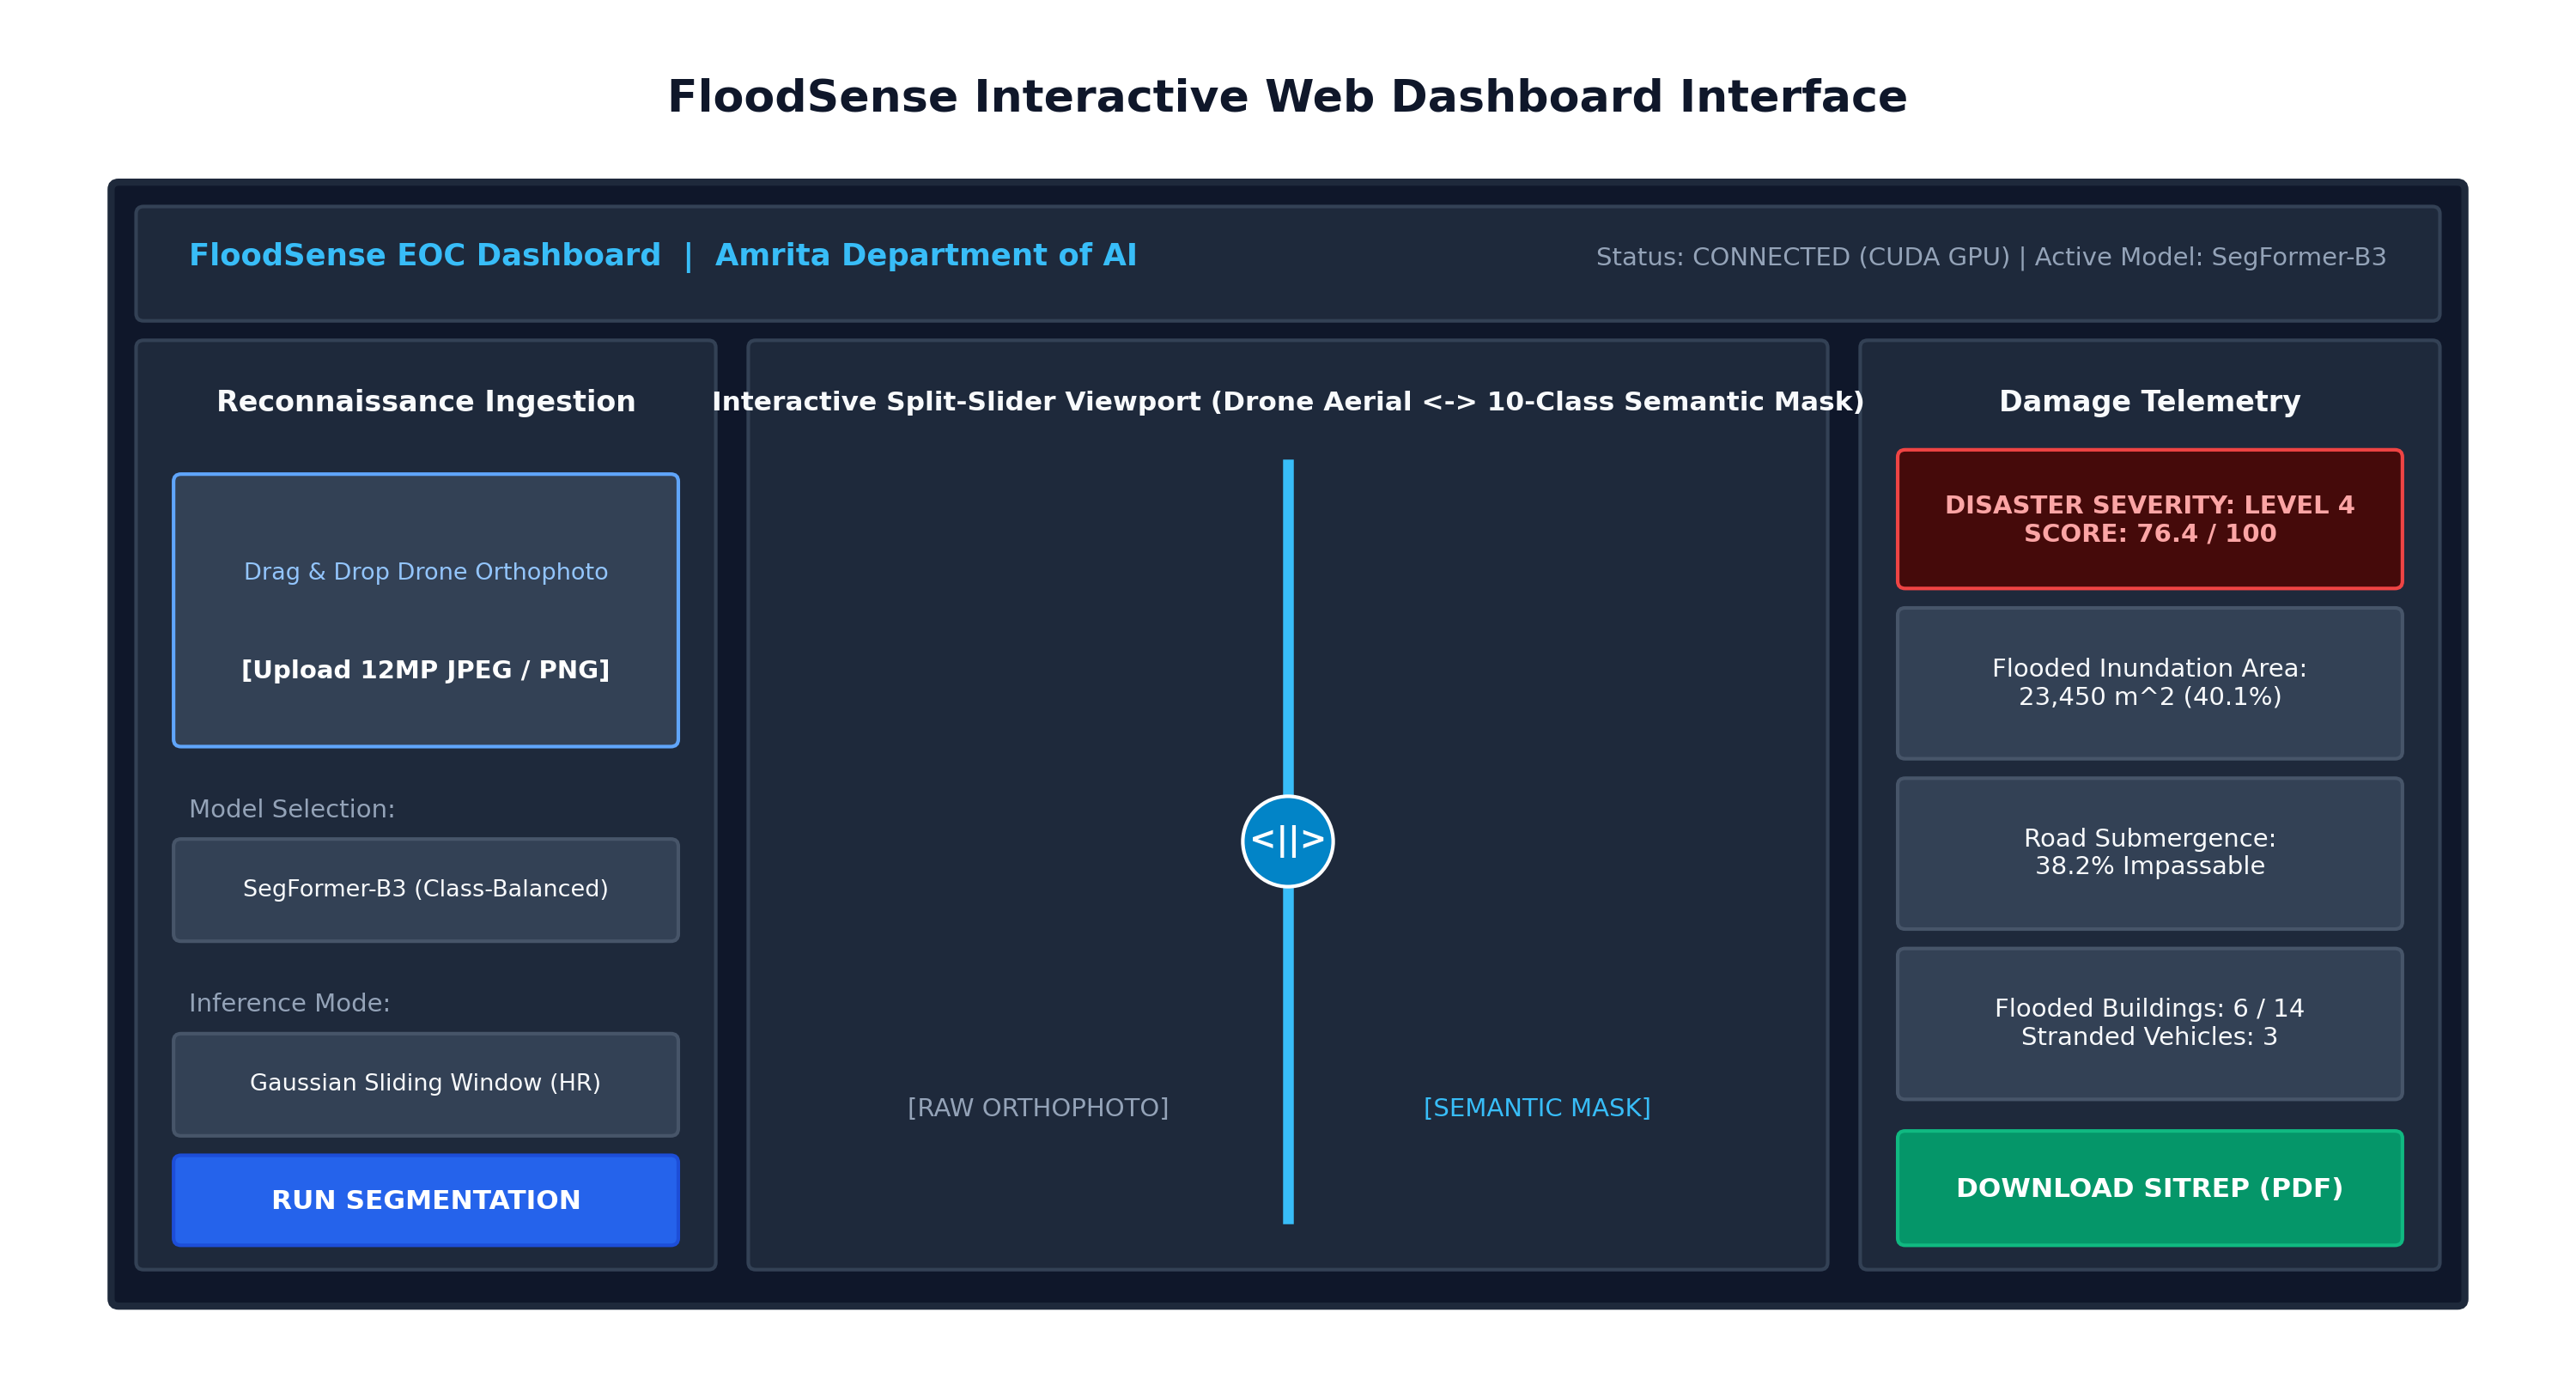
\includegraphics[width=0.92\textwidth]{images/fig7_dashboard_screenshot.png}
	\caption{Interactive Web Dashboard User Interface: Intuitive layout featuring split-slider visual overlay, real-time KPI damage cards, and one-click multi-format SITREP export.}
	\label{fig:dashboard_ui_mockup}
\end{figure}

Key interactive capabilities include:
\begin{itemize}
    \item \textbf{Split-Slider Comparison Viewer:} A GPU-accelerated canvas allowing operators to smoothly slide between raw drone imagery and color-coded semantic masks to visually verify flood boundaries against ground structures.
    \item \textbf{Real-Time Damage Telemetry Cards:} Prominent KPI cards displaying inundation surface area, submerged road percentages, building counts, and stranded vehicle alerts.
    \item \textbf{Dynamic SITREP Markdown Viewer:} An in-browser rich-text preview rendering tactical emergency action items, immediate 0--6 hour life-safety directives, and statutory NDMA/FEMA citation tags.
    \item \textbf{One-Click Multi-Format Export:} Direct download buttons triggering instantaneous generation of PDF, DOCX, and JSON files.
\end{itemize}

\section{Live Cloud Deployment Ecosystem}
To satisfy diverse organizational needs, FloodSense is packaged across three cloud deployment environments:
\begin{enumerate}
    \item \textbf{Production Cloud (Microsoft Azure):} Deployed on Microsoft Azure using Azure Container Apps (\texttt{floodsense-backend} in resource group \texttt{floodsense-rg}, East Asia) backed by container images built and pushed via Azure Container Registry (\texttt{floodsenseacr}). The containerized production backend runs Python 3.11 with Flask served via Gunicorn for enterprise production concurrency, paired with Supabase for secure authentication, relational data persistence, and cloud storage. The Azure Container Apps infrastructure provides automated health probes, managed SSL/TLS termination, configurable auto-scaling, and secure secret management to absorb concurrent ingestion traffic during emergency flood disasters.
    \item \textbf{Hugging Face Spaces Demonstration:} A lightweight, zero-configuration demonstration instance enabling researchers and civil defense agencies to test the model pipeline on public sample images without local installation.
    \item \textbf{GitHub Pages Documentation \& Client:} Automated via GitHub Actions (\texttt{.github/workflows/pages.yml}), hosting static project documentation, interactive architecture diagrams, and API schemas.
\end{enumerate}

\section{Practical Considerations for Emergency Operations Centers (EOCs)}
Deploying artificial intelligence systems in crisis response environments introduces practical constraints that theoretical models frequently ignore:
\begin{itemize}
    \item \textbf{Air-Gapped Field Edge Deployment:} In scenarios where external internet is destroyed, the entire FloodSense backend can be deployed locally on an NVIDIA Jetson AGX Orin or ruggedized GPU laptop. The deterministic fallback engine ensures that full SITREP compilation proceeds without requiring cloud API connections.
    \item \textbf{Inference Latency vs. Resolution Trade-off:} While standard $512 \times 512$ inference completes in $112\text{ ms}$, high-resolution sliding-window tiling on 12MP images requires $\approx 1.8\text{ seconds}$. The dashboard allows operators to toggle between "Fast Scout Mode" (512x512 for rapid preliminary screening) and "High-Resolution Survey Mode" (full sliding window for detailed infrastructure triage).
    \item \textbf{Data Privacy and Chain of Custody:} All processed aerial imagery, extracted coordinates, and generated SITREPs remain confined to local memory or customer-controlled cloud instances, ensuring strict compliance with governmental data sovereignty laws.
\end{itemize}

\section{Summary}
This chapter detailed the software engineering and deployment ecosystem of FloodSense. The modular REST API, interactive web dashboard, and cloud deployment on Microsoft Azure and Hugging Face ensure that high-accuracy deep learning models are immediately usable by frontline disaster responders. Chapter 8 concludes the thesis by summarizing primary research findings, assessing operational impacts, and identifying promising future research horizons.
